\chapter{La espectroscopia al servicio de la estructura}\label{ch:b1:structure-spectroscopy}

Un perfumista entrega al laboratorio un líquido incoloro que huele a piña
y pregunta qué es. Hace cincuenta años, la respuesta habría exigido
semanas de reacciones de degradación. Hoy lleva diez minutos: un análisis
elemental da la fórmula, un espectro infrarrojo nombra el grupo funcional
y un espectro de resonancia magnética nuclear de protón muestra cómo
están unidos los átomos. Este capítulo explica cómo se lee cada espectro
--- qué hace a una molécula la luz de cada región y qué rasgos de un
espectro contienen qué parte de la estructura --- y termina con esa
molécula de la piña.

\begin{recall}
El volumen escolar (años 11 y 12) midió \omterm{def:b1:structure-spectroscopy:absorbance}{absorbancias} con un
espectrofotómetro y usó la ley de Beer--Lambert para hallar
concentraciones, identificó grupos funcionales con tablas de bandas
infrarrojas y leyó espectros sencillos de RMN de protón (número de
señales, \omterm{def:b1:structure-spectroscopy:integration}{integración}, regla $n + 1$). Los enlaces sencillos, dobles y
triples y el enlace $\pi$ son los del
\cref{ch:b1:lewis-resonance-vsepr}.
\end{recall}

\section{Espectroscopia UV--visible: conjugación y color}

\begin{definition}[Absorbancia y ley de Beer--Lambert]\label{def:b1:structure-spectroscopy:absorbance}
Para una luz de intensidad $I_0$ que entra en una disolución e $I$ que
sale de ella, la \emph{absorbancia}\index{absorbancia} es
$A = \log(I_0/I)$. Para una disolución diluida de una sola especie
absorbente, $A = \varepsilon\,\ell\,c$ (la ley de Beer--Lambert), donde
$\ell$ es la longitud del trayecto, $c$ la concentración y $\varepsilon$
el \emph{coeficiente de absorción molar}\index{coeficiente de absorcion molar@coeficiente de absorción molar},
una propiedad de la especie a esa longitud de onda.
\end{definition}

Una molécula absorbe luz ultravioleta o visible cuando la energía de un
fotón coincide con la separación entre los niveles electrónicos ocupado
más alto y vacío más bajo de sus enlaces. En los enlaces $\sigma$ la
separación es grande y la absorción está muy en el ultravioleta; los
enlaces $\pi$ absorben más cerca del visible, y una cadena de enlaces
dobles y sencillos alternados absorbe a longitudes de onda tanto más
largas cuanto más larga es la cadena.

\begin{definition}[Sistema conjugado, cromóforo, máximo de absorción]\label{def:b1:structure-spectroscopy:conjugation}
Un \emph{sistema conjugado}\index{sistema conjugado} es una cadena de
átomos que llevan cada uno un orbital $p$ en un sistema $\pi$, como en los
enlaces dobles y sencillos alternados (buta-1,3-dieno, benceno). El grupo
de átomos responsable de una absorción es su
\emph{cromóforo}\index{cromoforo@cromóforo}; la longitud de onda a la que su \omterm{def:b1:structure-spectroscopy:absorbance}{absorbancia}
es máxima es el \emph{máximo de absorción}\index{maximo de absorcion@máximo de absorción},
$\lambda_{\max}$.
\end{definition}

Los niveles de un \omterm{def:b1:structure-spectroscopy:conjugation}{sistema conjugado} se extienden por toda la cadena y se
acercan entre sí a medida que la cadena crece, como los niveles de una
partícula en una caja más larga: $\lambda_{\max}$ aumenta con la
conjugación. El eteno y el butadieno solo absorben en el ultravioleta;
los once enlaces dobles conjugados del $\beta$-caroteno llevan la
absorción a la parte azul del visible. Una sustancia se ve del color
complementario de la luz que absorbe: al absorber el azul y el violeta, el
caroteno se ve naranja.

\begin{omfigure}
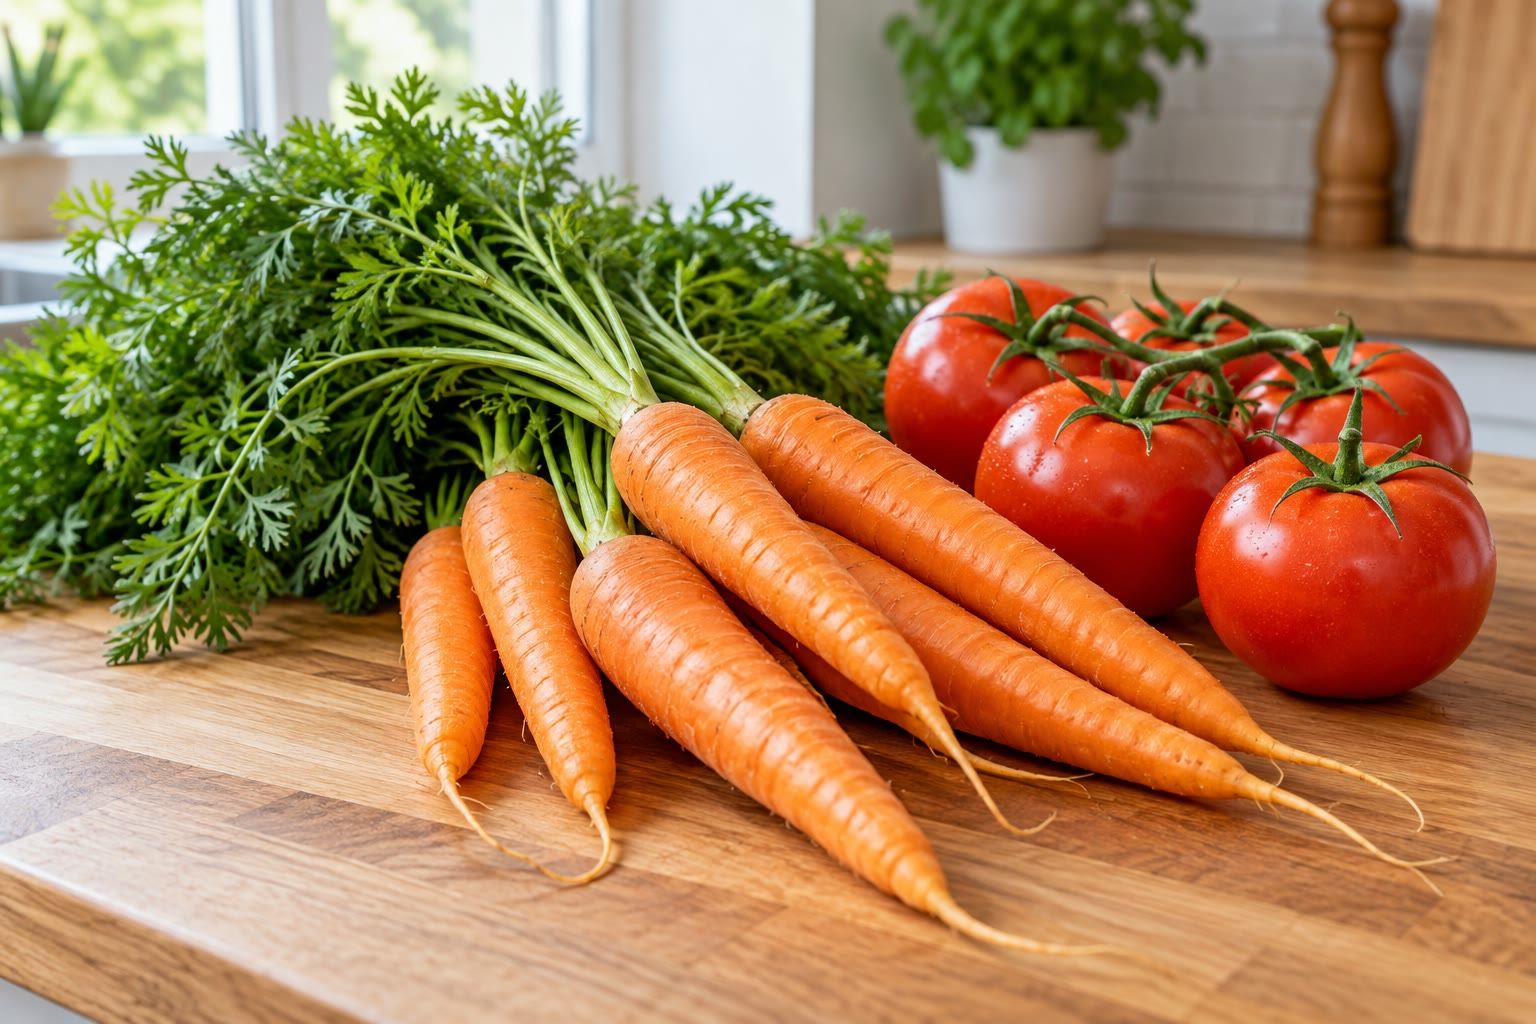
\includegraphics[width=0.55\linewidth]{images/book2/ai/b1-17-carrots-tomatoes.jpg}

{\small Las zanahorias y los tomates deben sus colores a moléculas
conjugadas largas, los carotenos y el licopeno, que absorben la luz azul y
verde y dejan pasar el naranja y el rojo.}
\end{omfigure}

\begin{omfigure}
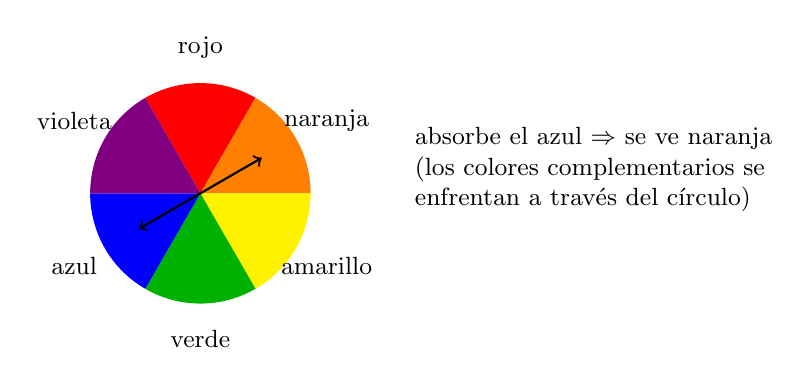
\begin{tikzpicture}[font=\small]
  \foreach \a/\c/\n in {90/red/rojo, 30/orange/naranja, -30/yellow/amarillo, -90/green!70!black/verde, -150/blue/azul, 150/violet/violeta} {
    \fill[\c] (0,0) -- (\a-30:1.4) arc[start angle=\a-30, end angle=\a+30, radius=1.4] -- cycle;
    \node at (\a:1.85) {\n};
  }
  \draw[<->, thick] (-150:0.9) -- (30:0.9);
  \node[align=left, anchor=west] at (2.6,0.3) {absorbe el azul $\Rightarrow$ se ve naranja\\(los colores complementarios se\\enfrentan a través del círculo)};
\end{tikzpicture}

{\small Un círculo cromático. El color que se ve es el complementario del
color absorbido: una disolución que absorbe en el azul se ve naranja.}
\end{omfigure}

\section{La espectroscopia infrarroja en profundidad}

\begin{definition}[Número de onda, transmitancia, región de la huella dactilar]\label{def:b1:structure-spectroscopy:wavenumber}
Los espectros infrarrojos se representan en función del \emph{número de
onda}\index{numero de onda@número de onda} $\tilde\nu = 1/\lambda$, en \unit{cm^{-1}},
proporcional a la energía del fotón. La ordenada es la
\emph{transmitancia}\index{transmitancia} $T = I/I_0$, en tanto por
ciento, de modo que las bandas apuntan hacia abajo. Por debajo de unos
\qty{1500}{cm^{-1}}, muchas bandas solapadas, características de la
molécula entera más que de un enlace, forman la \emph{región de la huella
dactilar}\index{region de la huella dactilar@región de la huella dactilar}.
\end{definition}

Un enlace absorbe la luz infrarroja a la frecuencia a la que vibra. Como
en dos masas unidas por un muelle, cuanto más rígido es el enlace y más
ligeros los átomos, mayor es el \omterm{def:b1:structure-spectroscopy:wavenumber}{número de onda}: los enlaces con el
hidrógeno (O--H, C--H), por encima de \qty{2800}{cm^{-1}}; los enlaces
triples, cerca de 2200; los dobles, hacia 1700--1600, y los sencillos
entre átomos más pesados, por debajo de 1300. La tabla da las posiciones
medidas para las moléculas de este capítulo, en \omterm{def:b1:extent-q-and-k:system}{fase} gaseosa, donde las
moléculas están aisladas.

\begin{omfigure}
\begin{tabular}{llr}
\hline
molécula & enlace & $\tilde\nu$ (\unit{cm^{-1}}) \\
\hline
etanol & O--H & 3666 \\
etanol & C--H & 2978 \\
etanol & C--O & 1060 \\
propanona & C=O & 1738 \\
ácido etanoico & O--H & 3582 \\
ácido etanoico & C=O & 1788 \\
etanoato de etilo & C=O & 1764 \\
etanoato de etilo & C--O & 1238 \\
\hline
\end{tabular}

\smallskip
{\small Máximos de las bandas en espectros infrarrojos en \omterm{def:b1:extent-q-and-k:system}{fase} gaseosa.
En los líquidos, los \omterm{def:b1:intermolecular-forces-solvents:hbond}{enlaces de hidrógeno} ensanchan las bandas O--H y las
desplazan a \omterm{def:b1:structure-spectroscopy:wavenumber}{números de onda} más bajos, y las bandas C=O de los ácidos
bajan cuando el ácido se empareja.}
% ledger: ir:ethanol-OH, ir:ethanol-CH, ir:ethanol-CO, ir:propanone-CO, ir:ethanoic-OH, ir:ethanoic-CO, ir:ethylethanoate-CO, ir:ethylethanoate-COC
\end{omfigure}

\begin{omfigure}
\begin{tikzpicture}
\begin{axis}[name=i1, width=0.86\linewidth, height=3.2cm, xmin=500, xmax=4000, x dir=reverse, ymin=0, ymax=105, ytick={0,50,100}, ylabel={$T$ (\%)}, tick label style={font=\scriptsize}, label style={font=\small}, xticklabels={}]
\addplot[omDef, thick] table[x=nu, y=T] {figdata/out/bachelor-1-spectra-ir-ethanol.dat};
\node[font=\scriptsize, anchor=west] at (axis cs:2600,25) {etanol};
\end{axis}
\begin{axis}[name=i2, at={(i1.south)}, anchor=north, yshift=-0.25cm, width=0.86\linewidth, height=3.2cm, xmin=500, xmax=4000, x dir=reverse, ymin=0, ymax=105, ytick={0,50,100}, ylabel={$T$ (\%)}, tick label style={font=\scriptsize}, label style={font=\small}, xticklabels={}]
\addplot[omProp, thick] table[x=nu, y=T] {figdata/out/bachelor-1-spectra-ir-propanone.dat};
\node[font=\scriptsize, anchor=west] at (axis cs:2600,25) {propanona};
\end{axis}
\begin{axis}[at={(i2.south)}, anchor=north, yshift=-0.25cm, width=0.86\linewidth, height=3.2cm, xmin=500, xmax=4000, x dir=reverse, ymin=0, ymax=105, ytick={0,50,100}, ylabel={$T$ (\%)}, tick label style={font=\scriptsize}, label style={font=\small}, xlabel={número de onda (\unit{cm^{-1}})}]
\addplot[omMeth, thick] table[x=nu, y=T] {figdata/out/bachelor-1-spectra-ir-ethanoic.dat};
\node[font=\scriptsize, anchor=west] at (axis cs:2600,25) {ácido etanoico};
\end{axis}
\end{tikzpicture}

{\small Espectros infrarrojos del etanol, la propanona y el ácido
etanoico, simulados a partir de las posiciones de banda medidas de la
tabla (alturas y anchuras de banda esquemáticas). La banda C=O cerca de
\qty{1750}{cm^{-1}} y la banda O--H por encima de \qty{3500}{cm^{-1}}
distinguen de un vistazo los tres grupos funcionales.}
\end{omfigure}

\section{RMN de protón: desplazamiento químico e integración}

En un campo magnético intenso, un protón tiene dos \omterm{def:b1:quantum-numbers:energy-level}{niveles de energía};
las ondas de radio de la frecuencia adecuada lo hacen pasar de uno a
otro. Esa frecuencia es proporcional al campo magnético que realmente
siente el protón, que los electrones que lo rodean reducen ligeramente.
Por eso los protones de entornos químicos distintos resuenan a
frecuencias ligeramente distintas.

\begin{definition}[Desplazamiento químico, apantallamiento, protones equivalentes]\label{def:b1:structure-spectroscopy:chemical-shift}
El \emph{desplazamiento químico}\index{desplazamiento quimico@desplazamiento químico} de un protón es
$\delta = (\nu - \nu_{\text{ref}})/\nu_0 \times 10^6$, en \unit{ppm}, donde
$\nu$ es su frecuencia de resonancia, $\nu_{\text{ref}}$ la de los
protones del tetrametilsilano y $\nu_0$ la frecuencia de trabajo del
espectrómetro. La reducción del campo en un núcleo debida a sus
electrones es su \emph{apantallamiento}\index{apantallamiento}: los
vecinos atractores de electrones (O, halógenos, C=O) desapantallan un
protón y elevan su $\delta$. Los \emph{protones
equivalentes}\index{protones equivalentes} son protones que se
intercambian por una simetría de la molécula o por una rotación rápida;
tienen el mismo desplazamiento.
\end{definition}

\begin{proposition}[El desplazamiento no depende del espectrómetro]\label{prop:b1:structure-spectroscopy:shift-field-independent}
El \omterm{def:b1:structure-spectroscopy:chemical-shift}{desplazamiento químico} de un protón es el mismo en espectrómetros de
campos distintos.
\end{proposition}

\begin{proof}
Tanto $\nu$ como $\nu_{\text{ref}}$ son proporcionales al campo aplicado
$B_0$ (cada una multiplicada por su propio factor de \omterm{def:b1:structure-spectroscopy:chemical-shift}{apantallamiento}), y
también lo es $\nu_0$. El cociente $(\nu - \nu_{\text{ref}})/\nu_0$ es,
por tanto, independiente de $B_0$. Las diferencias en hercios, en cambio,
crecen con el campo.
\end{proof}

\begin{definition}[Integración]\label{def:b1:structure-spectroscopy:integration}
La \emph{integración}\index{integracion@integración} de una señal es su área, que se lee
en el espectro como la altura de una curva escalonada; las áreas son
proporcionales a los números de protones que dan las señales.
\end{definition}

\section{El acoplamiento espín--espín}

\begin{definition}[Acoplamiento espín--espín, constante de acoplamiento, multiplete]\label{def:b1:structure-spectroscopy:coupling}
A través de los enlaces, el estado magnético de un protón modifica
ligeramente el campo que sienten los protones de los carbonos vecinos:
este \emph{acoplamiento espín--espín}\index{acoplamiento espin--espin@acoplamiento espín--espín} desdobla
cada señal en un \emph{multiplete}\index{multiplete} de líneas separadas
por la \emph{constante de acoplamiento}\index{constante de acoplamiento}
$J$, en hercios. Dos protones acoplados entre sí presentan la misma $J$;
los \omterm{def:b1:structure-spectroscopy:chemical-shift}{protones equivalentes} no desdoblan la señal unos de otros.
\end{definition}

\begin{proposition}[La regla \texorpdfstring{$n + 1$}{n + 1}]\label{prop:b1:structure-spectroscopy:n-plus-one}
Un protón (o un conjunto de \omterm{def:b1:structure-spectroscopy:chemical-shift}{protones equivalentes}) acoplado con la misma
$J$ a $n$ vecinos equivalentes da $n + 1$ líneas, separadas por $J$, de
intensidades relativas iguales a los coeficientes binomiales
$\binom{n}{k}$, de $k = 0$ a $n$ (la \emph{regla $n + 1$}\index{regla n + 1@regla $n + 1$}).
\end{proposition}

\begin{proof}
Cada vecino está en uno de dos estados de espín, que desplazan la línea
observada $+J/2$ o $-J/2$. Con $n$ vecinos, el desplazamiento es
$(k - n/2)J$, donde $k$ es el número de vecinos en el primer estado:
$n + 1$ valores, equiespaciados en $J$. Como los dos estados están casi
igual de poblados, las $2^n$ combinaciones son igual de probables, y que
$k$ de ellos estén en el primer estado ocurre de $\binom{n}{k}$ maneras.
\end{proof}

\begin{omfigure}
\begin{tikzpicture}[font=\small, x=0.85cm, y=0.5cm]
  % quartet: three neighbours, each split +-J/2 (J = 1.5 units)
  \draw[thick] (0,4) -- (0,3.4);
  \foreach \x in {-0.75,0.75} \draw (0,3.4) -- (\x,2.4);
  \foreach \a/\b in {-0.75/-1.5, -0.75/0, 0.75/0, 0.75/1.5} \draw (\a,2.4) -- (\b,1.4);
  \foreach \a/\b in {-1.5/-2.25, -1.5/-0.75, 0/-0.75, 0/0.75, 1.5/0.75, 1.5/2.25} \draw (\a,1.4) -- (\b,0.4);
  \foreach \x/\h in {-2.25/1, -0.75/3, 0.75/3, 2.25/1} {\draw[omDef, very thick] (\x,-2.6) -- (\x,{-2.6+0.7*\h}); \draw[dotted] (\x,0.4) -- (\x,{-2.6+0.7*\h});}
  \draw (-2.8,-2.6) -- (2.8,-2.6);
  \node at (0,-3.4) {cuadruplete 1\,:\,3\,:\,3\,:\,1 (\ce{-CH2-} junto a \ce{-CH3})};
  % triplet: two neighbours
  \begin{scope}[xshift=7.5cm]
  \draw[thick] (0,4) -- (0,3.4);
  \foreach \x in {-0.75,0.75} \draw (0,3.4) -- (\x,2.4);
  \foreach \a/\b in {-0.75/-1.5, -0.75/0, 0.75/0, 0.75/1.5} \draw (\a,2.4) -- (\b,1.4);
  \foreach \x/\h in {-1.5/1, 0/2, 1.5/1} {\draw[omProp, very thick] (\x,-2.6) -- (\x,{-2.6+0.7*\h}); \draw[dotted] (\x,1.4) -- (\x,{-2.6+0.7*\h});}
  \draw (-2.1,-2.6) -- (2.1,-2.6);
  \draw[<->] (-1.5,-0.6) -- (0,-0.6) node[midway, above, font=\scriptsize] {$J$};
  \node at (0,-3.4) {triplete 1\,:\,2\,:\,1 (\ce{-CH3} junto a \ce{-CH2-})};
  \end{scope}
\end{tikzpicture}

{\small Árboles de desdoblamiento. Cada vecino desdobla cada línea en dos,
separadas por $J$; las líneas que coinciden se suman y dan las
intensidades binomiales.}
\end{omfigure}

\begin{omfigure}
\begin{tikzpicture}
\begin{axis}[name=ea,
  width=0.86\linewidth, height=4.2cm, xmin=0.8, xmax=4.5, x dir=reverse, ymin=0, ymax=1.15,
  axis x line=bottom, axis y line=none, xlabel={$\delta$ (ppm)},
  tick label style={font=\scriptsize}, label style={font=\small}]
\addplot[omDef, thin] table[x=ppm, y=I] {figdata/out/bachelor-1-spectra-nmr-ethylethanoate.dat};
\node[font=\scriptsize, anchor=south] at (axis cs:4.12,0.75) {c, 2H};
\node[font=\scriptsize, anchor=west] at (axis cs:2.0,0.95) {s, 3H};
\node[font=\scriptsize, anchor=west] at (axis cs:1.15,0.8) {t, 3H};
\node[font=\small, anchor=north] at (axis cs:3.0,1.1) {\ce{CH3COOCH2CH3}};
\end{axis}
\begin{axis}[at={(ea.south)}, anchor=north, yshift=-1.3cm,
  width=0.86\linewidth, height=4.2cm, xmin=0.8, xmax=4.5, x dir=reverse, ymin=0, ymax=1.15,
  axis x line=bottom, axis y line=none, xlabel={$\delta$ (ppm)},
  tick label style={font=\scriptsize}, label style={font=\small}]
\addplot[omProp, thin] table[x=ppm, y=I] {figdata/out/bachelor-1-spectra-nmr-ethanol.dat};
\node[font=\scriptsize, anchor=south] at (axis cs:3.69,0.75) {c, 2H};
\node[font=\scriptsize, anchor=west] at (axis cs:2.55,0.6) {s, 1H};
\node[font=\scriptsize, anchor=west] at (axis cs:1.1,0.8) {t, 3H};
\node[font=\small, anchor=north] at (axis cs:2.9,1.1) {\ce{CH3CH2OH}};
\end{axis}
\end{tikzpicture}

{\small Espectros de RMN de protón del etanoato de etilo (arriba) y del
etanol (abajo) en \ce{CDCl3}, simulados a \qty{90}{MHz} a partir de
desplazamientos y \omterm{def:b1:structure-spectroscopy:coupling}{constantes de acoplamiento} medidos ($J = \qty{7.2}{Hz}$
y \qty{7.0}{Hz}). El cuadruplete (c) del \ce{OCH2} está desapantallado
por el oxígeno; en el etanol, el protón del OH, que se intercambia
rápidamente entre moléculas, no se acopla y su desplazamiento depende de
la concentración.}
% ledger: nmr:ethylethanoate-OCH2, nmr:ethylethanoate-COCH3, nmr:ethylethanoate-CH3, nmr:ethylethanoate-J, nmr:ethanol-CH2, nmr:ethanol-CH3, nmr:ethanol-OH, nmr:ethanol-J
\end{omfigure}

\begin{omfigure}
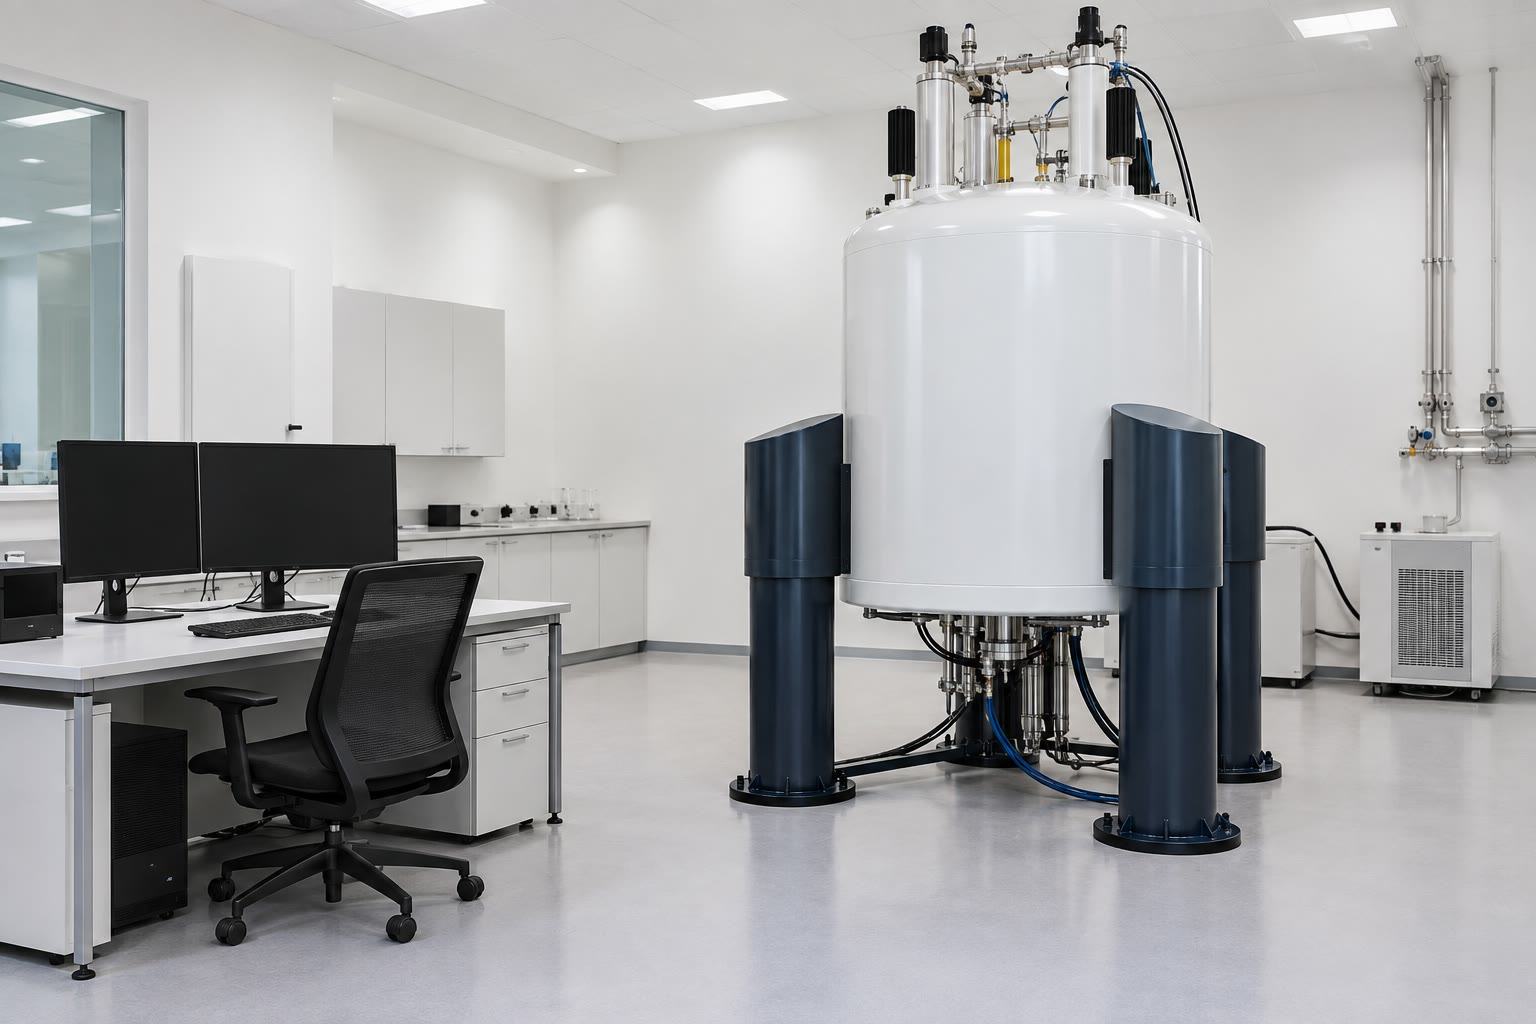
\includegraphics[width=0.5\linewidth]{images/book2/ai/b1-17-nmr.jpg}

{\small Un espectrómetro de RMN: el alto cilindro alberga un imán
superconductor enfriado con helio líquido; el tubo de muestra se baja
hasta su centro.}
\end{omfigure}

\section{Resolver una estructura}

\begin{definition}[Grado de insaturación]\label{def:b1:structure-spectroscopy:unsaturation}
El \emph{grado de insaturación}\index{grado de insaturacion@grado de insaturación} de una fórmula
es el número de anillos más el número de enlaces $\pi$ de la molécula.
\end{definition}

\begin{proposition}[Grado de insaturación a partir de la fórmula]\label{prop:b1:structure-spectroscopy:unsaturation-formula}
Para una molécula $\mathrm{C}_c\mathrm{H}_h\mathrm{N}_n\mathrm{O}_o\mathrm{X}_x$
(X, un halógeno), el \omterm{def:b1:structure-spectroscopy:unsaturation}{grado de insaturación} es
\[
  D = \frac{2c + 2 + n - h - x}{2} .
\]
\end{proposition}

\begin{proof}
Una cadena abierta de $c$ carbonos con solo enlaces sencillos lleva
$2c + 2$ hidrógenos. Cada anillo o enlace $\pi$ quita dos de ellos. Un
oxígeno divalente insertado en una cadena no cambia nada; un nitrógeno
trivalente aporta un hidrógeno más; un halógeno ocupa el lugar de un
hidrógeno. Contar los hidrógenos que faltan y dividir por dos da $D$.
\end{proof}

\begin{method}[Resolver una estructura]\label{met:b1:structure-spectroscopy:solve-structure}
\begin{enumerate}
  \item A partir de la fórmula, se calcula $D$.
  \item A partir del espectro IR, se hallan los grupos funcionales (C=O,
        O--H, N--H, C--O) y la ausencia de otros.
  \item A partir del espectro de RMN: número de señales (conjuntos de
        \omterm{def:b1:structure-spectroscopy:chemical-shift}{protones equivalentes}), \omterm{def:b1:structure-spectroscopy:integration}{integraciones} (protones por conjunto),
        desplazamientos (grupos vecinos), multiplicidades (número de
        vecinos según la regla $n + 1$), \omterm{def:b1:structure-spectroscopy:coupling}{constantes de acoplamiento} (qué
        señales son vecinas).
  \item Se construyen fragmentos, se unen y se comprueba cada pico frente
        a la estructura propuesta; se descartan los isómeros que no
        concuerdan.
\end{enumerate}
\end{method}

\section{Ejercicios}

\begin{exercise}[$\star$]\label{exo:b1:structure-spectroscopy:1}
Una disolución de un colorante de \qty{2.0e-5}{mol/L} en una cubeta de
\qty{1.00}{cm} tiene una \omterm{def:b1:structure-spectroscopy:absorbance}{absorbancia} de 0.64 en su \omterm{def:b1:structure-spectroscopy:conjugation}{máximo de absorción}.
Calcúlense $\varepsilon$ y la \omterm{def:b1:structure-spectroscopy:absorbance}{absorbancia} de una disolución tres veces
más concentrada.
\end{exercise}

\begin{exercise}[$\star$]\label{exo:b1:structure-spectroscopy:2}
Calcúlese el \omterm{def:b1:structure-spectroscopy:unsaturation}{grado de insaturación} de \ce{C6H6}, \ce{C4H8O2},
\ce{C3H7NO}, \ce{C2H3Cl} y \ce{C10H14O} (la carvona). Propóngase una
estructura para cada uno.
\end{exercise}

\begin{exercise}[$\star$]\label{exo:b1:structure-spectroscopy:3}
¿Cuántas señales de protón, y con qué \omterm{def:b1:structure-spectroscopy:integration}{integraciones}, dan la propanona,
el ácido etanoico, el 2-metilpropano y el 1,2-dicloroetano?
\end{exercise}

\begin{exercise}[$\star$]\label{exo:b1:structure-spectroscopy:4}
Una señal está a \qty{1460}{Hz} del tetrametilsilano en un espectrómetro
de \qty{400}{MHz}. ¿Cuál es su desplazamiento? ¿A cuántos hercios estaría
a \qty{90}{MHz}? ¿Por qué los campos altos separan mejor los \omterm{def:b1:structure-spectroscopy:coupling}{multipletes}?
\end{exercise}

\begin{exercise}[$\star\star$]\label{exo:b1:structure-spectroscopy:5}
Predígase la multiplicidad de cada señal del 1-bromopropano,
\ce{CH3CH2CH2Br}, suponiendo \omterm{def:b1:structure-spectroscopy:coupling}{constantes de acoplamiento} iguales, y las
intensidades relativas de las líneas de la señal central.
\end{exercise}

\begin{exercise}[$\star\star$]\label{exo:b1:structure-spectroscopy:6}
¿En qué difieren los espectros IR del etanol, la propanona y el ácido
etanoico entre 1700 y \qty{3700}{cm^{-1}}? ¿Qué compuesto da a la vez una
banda C=O y una banda O--H?
\end{exercise}

\begin{exercise}[$\star\star$]\label{exo:b1:structure-spectroscopy:7}
Dos isómeros \ce{C4H8O2}: el etanoato de etilo y el propanoato de metilo.
Predíganse sus espectros de RMN (desplazamientos aproximados,
multiplicidades, \omterm{def:b1:structure-spectroscopy:integration}{integraciones}) y dígase cómo distinguirlos.
\end{exercise}

\begin{exercise}[$\star\star$]\label{exo:b1:structure-spectroscopy:8}
Con el espectro simulado del etanoato de etilo, léase la separación entre
dos líneas del cuadruplete en ppm y conviértase en hercios (el espectro
está simulado a \qty{90}{MHz}). Compárese con el triplete.
\end{exercise}

\begin{exercise}[$\star\star$]\label{exo:b1:structure-spectroscopy:9}
Un compuesto \ce{C3H6O} presenta una banda IR intensa a
\qty{1738}{cm^{-1}} y una sola señal de RMN. Identifíquese. ¿Qué isómero
presentaría una banda cerca de \qty{2720}{cm^{-1}} y una señal cerca de
\qty{9.8}{ppm}?
\end{exercise}

\begin{exercise}[$\star\star\star$]\label{exo:b1:structure-spectroscopy:10}
Demuéstrese la regla $n + 1$ en la forma siguiente: un protón acoplado a
dos conjuntos distintos de vecinos, $n_1$ con $J_1$ y $n_2$ con $J_2$, da
$(n_1 +
1)(n_2 + 1)$ líneas. Cuando $J_1 = J_2$, ¿cuántas líneas distintas
quedan? Aplíquese al \ce{CH2} central del 1-bromopropano.
\end{exercise}

\begin{exercise}[$\star\star\star$]\label{exo:b1:structure-spectroscopy:11}
Un compuesto \ce{C4H10O} no da ninguna banda IR entre 1700 y 1800, pero
sí una banda ancha cerca de \qty{3350}{cm^{-1}} en el líquido, y un
espectro de RMN con un doblete (6H), un \omterm{def:b1:structure-spectroscopy:coupling}{multiplete} (1H), un doblete (2H)
y un singlete ancho (1H). Hállese la estructura.
\end{exercise}

\begin{exercise}[$\star\star\star$]\label{exo:b1:structure-spectroscopy:12}
Demuéstrese que la \omterm{def:b1:structure-spectroscopy:absorbance}{absorbancia} de una mezcla de dos especies cumple
$A = \ell(\varepsilon_1c_1
+ \varepsilon_2c_2)$, y explíquese cómo dan las medidas a dos longitudes
de onda las dos concentraciones.
\end{exercise}

\section{Problema: la molécula de la piña}

\begin{problem}[{Problema de fin de semana --- análisis por combustión y
densidad del vapor, el espectro infrarrojo, el espectro de RMN de protón,
y la estructura y la masa molar del éster con olor a piña}]
\label{pb:b1:structure-spectroscopy:1}
La sustancia desconocida es un líquido que solo contiene C, H y O. La
combustión de \qty{0.2500}{g} da \qty{0.5690}{g} de dióxido de carbono y
\qty{0.2328}{g} de agua. Su vapor tiene una densidad de \qty{3.74}{g/L} a
\qty{100}{\celsius} y \qty{1.000}{bar}. Bandas IR en \omterm{def:b1:extent-q-and-k:system}{fase} gaseosa: 2982,
1754 y \qty{1182}{cm^{-1}} (intensa), ninguna por encima de
\qty{3100}{cm^{-1}}. RMN de protón (\ce{CDCl3}): 4.13 (c, 2H, $J = \qty{7.2}{Hz}$),
2.28 (t, 2H), 1.66 (sextuplete, 2H), 1.25 (t, 3H, $J = \qty{7.2}{Hz}$),
0.95 (t, 3H) ppm. $M$: C 12.0, H 1.0, O \qty{16.0}{g/mol}; $R =
\qty{8.314}{J/(K.mol)}$.
% ledger: ir:ethylbutanoate-CH, ir:ethylbutanoate-CO, ir:ethylbutanoate-COC, nmr:ethylbutanoate-OCH2, nmr:ethylbutanoate-CH2CO, nmr:ethylbutanoate-CH2, nmr:ethylbutanoate-OCH2CH3, nmr:ethylbutanoate-CH3, nmr:ethylbutanoate-J

\begin{center}
\begin{tikzpicture}
\begin{axis}[width=0.86\linewidth, height=4.0cm, xmin=0.6, xmax=4.5, x dir=reverse, ymin=0, ymax=1.15,
  axis x line=bottom, axis y line=none, xlabel={$\delta$ (ppm)},
  tick label style={font=\scriptsize}, label style={font=\small}]
\addplot[omDef, thin] table[x=ppm, y=I] {figdata/out/bachelor-1-spectra-nmr-ethylbutanoate.dat};
\end{axis}
\end{tikzpicture}
\end{center}

\medskip
\noindent\textbf{Parte I --- La fórmula.}
\begin{enumerate}
  \item Calcúlese la masa de carbono de la muestra.
  \item Calcúlese la masa de hidrógeno.
  \item Dedúzcase la masa de oxígeno.
  \item Calcúlense los porcentajes en masa de C, H y O.
  \item Hállese la fórmula empírica.
  \item A partir de la densidad del vapor, calcúlese la masa molar (gas
        ideal).
  \item Dense la fórmula molecular y su \omterm{def:b1:structure-spectroscopy:unsaturation}{grado de insaturación}.
\end{enumerate}

\medskip
\noindent\textbf{Parte II --- El espectro infrarrojo.}
\begin{enumerate}[resume]
  \item Asígnese la banda de \qty{1754}{cm^{-1}}.
  \item ¿Qué excluye la ausencia de bandas por encima de
        \qty{3100}{cm^{-1}}?
  \item Asígnese la banda intensa de \qty{1182}{cm^{-1}}.
  \item Asígnese la banda de \qty{2982}{cm^{-1}}.
  \item Con el \omterm{def:b1:structure-spectroscopy:unsaturation}{grado de insaturación}, ¿qué familia de compuestos queda?
        ¿Por qué no un ácido carboxílico, una cetona con un éter o un
        diol cíclico?
\end{enumerate}

\medskip
\noindent\textbf{Parte III --- El espectro de RMN.}
\begin{enumerate}[resume]
  \item ¿Cuántos conjuntos de \omterm{def:b1:structure-spectroscopy:chemical-shift}{protones equivalentes} hay? Compruébese la
        \omterm{def:b1:structure-spectroscopy:integration}{integración} total.
  \item Interprétese el cuadruplete de 4.13 ppm: vecinos y entorno.
  \item Interprétese el triplete de 1.25 ppm. ¿Por qué tienen ambos la
        misma $J$?
  \item Interprétese el triplete de 2.28 ppm.
  \item Interprétese el sextuplete de 1.66 ppm.
  \item Interprétese el triplete de 0.95 ppm.
  \item Constrúyanse los dos fragmentos que describen estas señales.
  \item ¿Por qué las señales de 4.13 y 2.28 ppm son las más
        desapantalladas?
\end{enumerate}

\medskip
\noindent\textbf{Parte IV --- La estructura.}
\begin{enumerate}[resume]
  \item Únanse los fragmentos a través del grupo éster: dos
        posibilidades. ¿Cuál es coherente con los desplazamientos?
  \item Explíquese por qué no encaja el propanoato de propilo.
  \item Explíquese por qué no encaja el etanoato de butilo.
  \item Nómbrese el compuesto y dibújese su estructura.
  \item Compruébense cada banda IR y cada señal de RMN frente a la
        estructura.
  \item Dese la masa molar de la molécula de la piña.
\end{enumerate}
\end{problem}
